\chapter{非线性控制系统分析}

\section{非线性特性}

\subsection{非线性特点}

非线性和线性系统的区别很大，其特点主要体现在以下的几点：
\begin{enumerate}
    \item 不满足叠加定理
    \item 其稳定性的分析更加复杂，系统的初值对于稳定性的影响比较大
    \item 在非线性系统中，存在自激振荡，表现为振荡特性，且在振幅较大的时候会慢慢振幅变小，在振幅较小的时候会慢慢变大
    \item 混沌现象：有些非线性系统的输出对初始条件极为铭感。即使具有确定性的、十分精确的模型，也不能语言系统初始条件变化时的输出变化，这个现象就被称为混沌现象
\end{enumerate}

\subsection{典型非线性特性}

我们主要讨论以下几种比较典型的非线性特性：
\begin{enumerate}
    \item 饱和特性
    \item 死区特性
    \item 滞环特性
    \item 继电特性
    \item 变增益特性
\end{enumerate}
\subsubsection{饱和特性}

饱和特性的示意图如下：
\begin{center}
    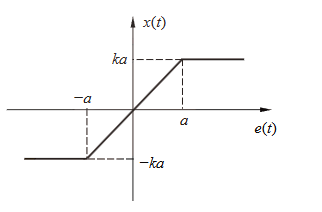
\includegraphics[width = .2\textwidth]{note/nonlinear system/figure/1.png}
\end{center}

其表达式可以写成以下的形式：
\[
x(t)=
\begin{cases}
k e(t), & |e(t)| \le a,\\
k a \operatorname{sgn}(e(t)), & |e(t)| > a.
\end{cases}
\]

\subsubsection{死区特性}

死区特性的示意图如下：
\begin{center}
    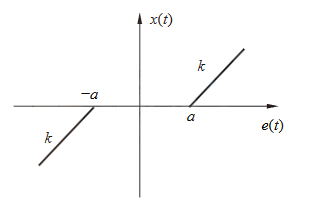
\includegraphics[width = .2\textwidth]{note/nonlinear system/figure/2.png}
\end{center}

其表达式可以写成以下的形式：
\[
x(t)=
\begin{cases}
k\bigl(e(t)+a\bigr), & e(t)<-a,\\
0, & |e(t)|<a,\\
k\bigl(e(t)-a\bigr), & e(t)>a.
\end{cases}
\]

\subsubsection{滞环特性}

滞环特性的示意图如下：
\begin{center}
    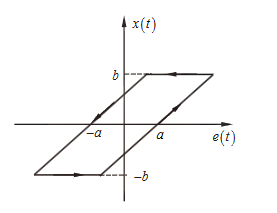
\includegraphics[width = .2\textwidth]{note/nonlinear system/figure/3.png}
\end{center}

其表达式可以写成以下的形式：
\[
x(t)=
\begin{cases}
k\bigl[e(t)-a\bigr], & \dot{x}(t)>0,\\
b\operatorname{sgn}\bigl(e(t)\bigr), & \dot{x}(t)=0,\\
k\bigl[e(t)+a\bigr], & \dot{x}(t)<0.
\end{cases}
\]

\subsubsection{继电特性}

继电特性的示意图如下：
\begin{center}
    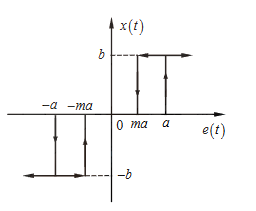
\includegraphics[width = .2\textwidth]{note/nonlinear system/figure/4.png}
\end{center}

其表达式可以写成以下的形式：
\[
x(t)=
\begin{cases}
0, & -ma < e(t) < a,\ \dot{e}(t)>0,\\
0, & -a < e(t) < ma,\ \dot{e}(t)<0,\\
b\operatorname{sgn}\bigl(e(t)\bigr), & |e(t)| \ge a,\\
b, & e(t) \ge ma,\ \dot{e}(t)<0,\\
-b, & e(t) \le -ma,\ \dot{e}(t)>0.
\end{cases}
\]

可以发现，这里面$m$和$a$对于特性的影响比较大，当$m$和$a$分别取特定值的时候可以得到以下的几种特殊情况：
\begin{enumerate}
    \item 当$a = 0$时可以得到理想继电器：
    \begin{center}
        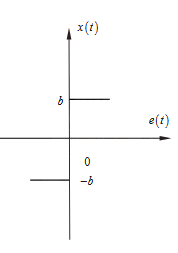
\includegraphics[width = .2\textwidth]{note/nonlinear system/figure/5.png}
    \end{center}
    \item 当$m = 1$时可以得到带死区的继电器：
    \begin{center}
        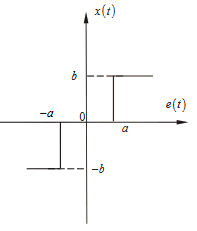
\includegraphics[width = .2\textwidth]{note/nonlinear system/figure/6.png}
    \end{center}
    \item 当$m = -1$时可以得到带滞环的继电器：
    \begin{center}
        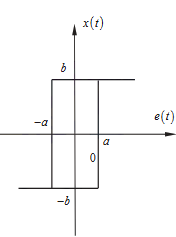
\includegraphics[width = .2\textwidth]{note/nonlinear system/figure/7.png}
    \end{center}
\end{enumerate}

\subsubsection{变增益特性}

变增益特性的示意图如下：
\begin{center}
    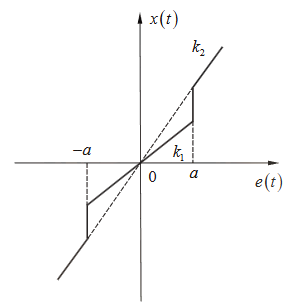
\includegraphics[width = .2\textwidth]{note/nonlinear system/figure/8.png}
\end{center}

其表达式可以写成以下形式：
\[
x(t)=
\begin{cases}
k_1 e(t), & |e(t)| < a,\\
k_2 e(t), & |e(t)| > a.
\end{cases}
\]

\section{描述函数法}

对于一个线性系统，我们可以通过写出其传递函数来给出输入和输出的具体关系，通过输入来计算输出。可是，对于非线性系统，我们没有办法直接写出其传递函数，此时应该怎么办呢？

我们可以通过类比线性系统\hyperref[frequency-characteristics]{频率特性}来给出非线性系统的近似的传递函数，具体如下：

假设一个时不变系统如下图所示：
\begin{center}
    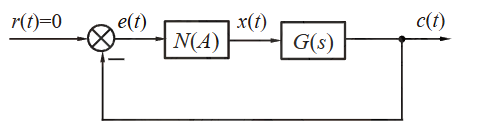
\includegraphics[width = .4\textwidth]{note/nonlinear system/figure/9.png}
\end{center}
且系统的误差为$e(t) = A \sin \omega t$，此时经过非线性部分之后得到的输出一定为周期信号（输入经过时不变系统不改变周期性），故我们可以通过Fourier级数展开将$x(t)$写成如下的形式：
\[
\begin{aligned}
x(t) &= A_0 + \sum_{n=1}^{\infty}
\left(A_n \cos n\omega t + B_n \sin n\omega t\right) \\
&= A_0 + \sum_{n=1}^{\infty}
X_n \sin\left(n\omega t + \varphi_n\right)
\end{aligned}
\]
其中：
\[
\begin{aligned}
A_0 &= \frac{1}{2\pi}\int_{0}^{2\pi} x(t)\,\mathrm{d}(\omega t) \\
A_n &= \frac{1}{\pi}\int_{0}^{2\pi} x(t)\cos n\omega t\,\mathrm{d}(\omega t) \\
B_n &= \frac{1}{\pi}\int_{0}^{2\pi} x(t)\sin n\omega t\,\mathrm{d}(\omega t) \\
X_n &= \sqrt{A_n^2+B_n^2} \\
\varphi_n &= \arctan \frac{A_n}{B_n}
\end{aligned}
\]
但此时的输出仍然很复杂，且有很多谐波叠加，为了写成类似频率特性的形式，我们引入以下两个假设，使其近似为频率特性的形式：
\begin{enumerate}
    \item \textbf{奇对称性}：即正弦输入下的输出$x(t)$为$t$的奇对称函数，$x(t + \frac{\pi}{\omega}) = - x(t)$，以保证非线性环节的正弦响应不含有常值分量，即$A_0 = 0$

    进一步地，若$x(t)$为奇函数，此时我们可以得到$A_i = 0, B_1 = \frac{4}{\pi}\int_0^{\frac{\pi}{2}} x(t) \sin \omega t d \omega t$
    \item \textbf{线性环节低通滤波特性良好}：在整个系统中，线性环节低通滤波特性良好，意味着在正弦输入情况下，实际输出中高次谐波分量将被大大削弱。只有在这种条件下，实际输出中基波分量才能较精确地近似代替正弦输入信号下的实际输出。当然，描述函数法分析的精度也直接取决于线性环节的低通滤波特性，低通滤波特性越好，相应的分析精度也越高。
\end{enumerate}
有了以上两个假设，我们可以将非线性环节的输出写成以下的形式：
\[
\begin{aligned}
x(t) \approx x_1(t)
&= A_1 \cos \omega t + B_1 \sin \omega t \\
&= X_1 \sin\left(\omega t+\varphi_1\right)
\end{aligned}
\]
此时非线性环节的描述函数为：
\[
\begin{aligned}
N(A)
&= \frac{X_1}{A} e^{j\varphi_1} \\
&= \frac{\sqrt{A_1^2+B_1^2}}{A}
e^{j\arctan\frac{A_1}{B_1}} \\
&= \frac{B_1}{A} + j\frac{A_1}{A}
\end{aligned}
\]

\subsection{典型非线性特性的描述函数}

\subsubsection{理想继电特性}
为了更好地看出$x(t)$的图像，我们将$e(t)$的图像竖直放在$x(e)$的下方，如下图所示：
\begin{center}
    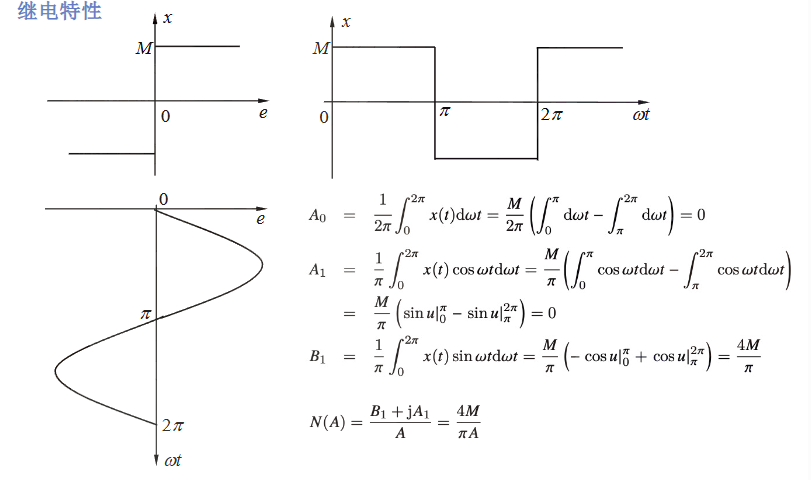
\includegraphics[width = .5\textwidth]{note/nonlinear system/figure/10.png}
\end{center}
由图可知：
\[
\begin{aligned}
A_0
&= \frac{1}{2\pi}\int_{0}^{2\pi} x(t)\,\mathrm{d}\omega t
= \frac{M}{2\pi}\left(\int_{0}^{\pi}\mathrm{d}\omega t
-\int_{\pi}^{2\pi}\mathrm{d}\omega t\right)=0 \\
A_1
&= \frac{1}{\pi}\int_{0}^{2\pi} x(t)\cos\omega t\,\mathrm{d}\omega t
= \frac{M}{\pi}\left(\int_{0}^{\pi}\cos\omega t\,\mathrm{d}\omega t
-\int_{\pi}^{2\pi}\cos\omega t\,\mathrm{d}\omega t\right) \\
&= \frac{M}{\pi}\left(\sin\omega t\big|_{0}^{\pi}
-\sin\omega t\big|_{\pi}^{2\pi}\right)=0 \\
B_1
&= \frac{1}{\pi}\int_{0}^{2\pi} x(t)\sin\omega t\,\mathrm{d}\omega t
= \frac{M}{\pi}\left(-\cos\omega t\big|_{0}^{\pi}
+\cos\omega t\big|_{\pi}^{2\pi}\right)
= \frac{4M}{\pi} \\
N(A)
&= \frac{B_1+jA_1}{A}
= \frac{4M}{\pi A}
\end{aligned}
\]

\subsubsection{死区特性}
同样的，也可以给出示意图如下：
\begin{center}
    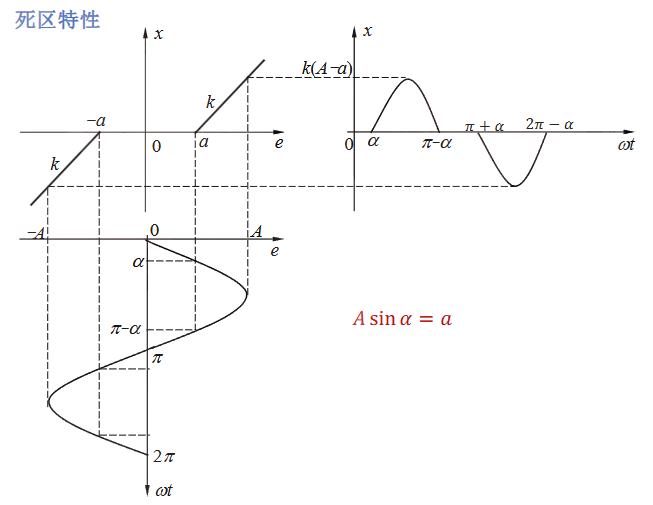
\includegraphics[width = .5\textwidth]{note/nonlinear system/figure/11.png}
\end{center}
由图：由于 $x(t)$ 为单位且奇对称的，并且 $x(t)\sin\omega t$ 具有 $1/4$ 波对称性，
所以有 $A_0=0, A_1=0$，并且
\[
\begin{aligned}
B_1
&= \frac{1}{\pi}\int_{0}^{2\pi} x(t)\sin\omega t\,\mathrm{d}(\omega t) \\
&= \frac{4}{\pi}\int_{\alpha}^{\frac{\pi}{2}}
k\left(A\sin\omega t-a\right)\sin\omega t\,\mathrm{d}(\omega t) \\
&= \frac{2kA}{\pi}
\left[
\frac{\pi}{2}
-\arcsin\frac{a}{A}
-\frac{a}{A}\sqrt{1-\left(\frac{a}{A}\right)^2}
\right],
\qquad A>a
\end{aligned}
\]

此时，可得死区特性的描述函数为
\[
N(A)=\frac{B_1}{A}
=\frac{2k}{\pi}
\left[
\frac{\pi}{2}
-\arcsin\frac{a}{A}
-\frac{a}{A}\sqrt{1-\left(\frac{a}{A}\right)^2}
\right],
\qquad A\ge a
\]

\subsubsection{饱和特性}
饱和特性的示意图如下：
\begin{center}
    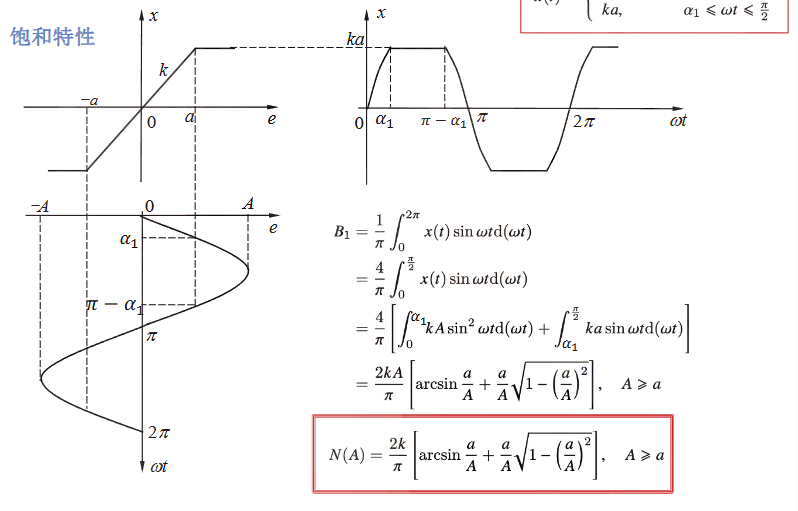
\includegraphics[width = .5\textwidth]{note/nonlinear system/figure/12.png}
\end{center}
由图可知：
\[
\begin{aligned}
A_1 & = A_0 = 0\\
B_1
&= \frac{1}{\pi}\int_{0}^{2\pi} x(t)\sin\omega t\,\mathrm{d}(\omega t) \\
&= \frac{4}{\pi}\int_{0}^{\frac{\pi}{2}} x(t)\sin\omega t\,\mathrm{d}(\omega t) \\
&= \frac{4}{\pi}
\left[
\int_{0}^{\alpha_1} kA\sin^2\omega t\,\mathrm{d}(\omega t)
+\int_{\alpha_1}^{\frac{\pi}{2}} ka\sin\omega t\,\mathrm{d}(\omega t)
\right] \\
&= \frac{2kA}{\pi}
\left[
\arcsin\frac{a}{A}
+\frac{a}{A}\sqrt{1-\left(\frac{a}{A}\right)^2}
\right],
\qquad A\ge a
\end{aligned}
\]

\[
N(A)=\frac{2k}{\pi}
\left[
\arcsin\frac{a}{A}
+\frac{a}{A}\sqrt{1-\left(\frac{a}{A}\right)^2}
\right],
\qquad A\ge a
\]

\subsubsection{滞环特性}
滞环特性的示意图如下：
\begin{center}
    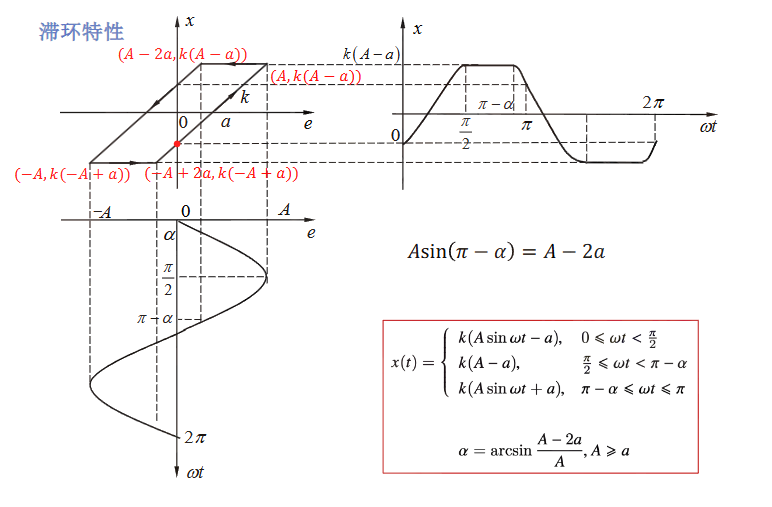
\includegraphics[width = .5\textwidth]{note/nonlinear system/figure/13.png}
\end{center}

由图：
\[
\begin{aligned}
A_1
&= \frac{1}{\pi}\int_{0}^{2\pi} x(t)\cos\omega t\,\mathrm{d}(\omega t) \\
&= \frac{2}{\pi}
\left[
\int_{0}^{\frac{\pi}{2}} k(A\sin\omega t-a)\cos\omega t\,\mathrm{d}(\omega t)
+\int_{\frac{\pi}{2}}^{\pi-\alpha} k(A-a)\cos\omega t\,\mathrm{d}(\omega t)\right. \\
&\qquad\left.
+\int_{\pi-\alpha}^{\pi} k(A\sin\omega t+a)\cos\omega t\,\mathrm{d}(\omega t)
\right] \\
&= \frac{4ka}{\pi}\left(\frac{a}{A}-1\right),
\qquad A\ge a
\end{aligned}
\]

\[
\begin{aligned}
B_1
&= \frac{1}{\pi}\int_{0}^{2\pi} x(t)\sin\omega t\,\mathrm{d}(\omega t) \\
&= \frac{2}{\pi}
\left[
\int_{0}^{\frac{\pi}{2}} k(A\sin\omega t-a)\sin\omega t\,\mathrm{d}(\omega t)
+\int_{\frac{\pi}{2}}^{\pi-\alpha} k(A-a)\sin\omega t\,\mathrm{d}(\omega t)\right. \\
&\qquad\left.
+\int_{\pi-\alpha}^{\pi} k(A\sin\omega t+a)\sin\omega t\,\mathrm{d}(\omega t)
\right] \\
&= \frac{kA}{\pi}
\left[
\frac{\pi}{2}
+\arcsin\left(1-\frac{2a}{A}\right)
+2\left(1-\frac{2a}{A}\right)
\sqrt{\frac{a}{A}\left(1-\frac{a}{A}\right)}
\right],
\qquad A\ge a
\end{aligned}
\]

\[
\begin{aligned}
N(A)
&= \frac{B_1}{A}+j\frac{A_1}{A} \\
&= \frac{k}{\pi}
\left[
\frac{\pi}{2}
+\arcsin\left(1-\frac{2a}{A}\right)
+2\left(1-\frac{2a}{A}\right)
\sqrt{\frac{a}{A}\left(1-\frac{a}{A}\right)}
\right] \\
&\qquad
+j\frac{4ka}{\pi A}\left(\frac{a}{A}-1\right),
\qquad A\ge a
\end{aligned}
\]

\subsubsection{继电特性}
继电特性的示意图如下：
\begin{center}
    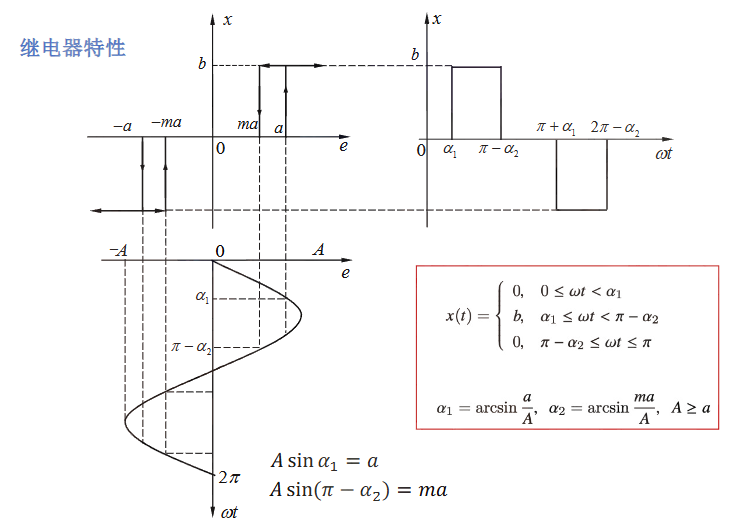
\includegraphics[width = .5\textwidth]{note/nonlinear system/figure/14.png}
\end{center}
由 $x(t)$ 正、负半波对称性知，$A_0=0$。计算 $A_1$，$B_1$ 得
\[
\begin{aligned}
A_1
&= \frac{1}{\pi}\int_{0}^{2\pi}x(t)\cos\omega t\,\mathrm{d}(\omega t) \\
&= \frac{2}{\pi}\int_{\alpha_1}^{\pi-\alpha_2} b\cos\omega t\,\mathrm{d}(\omega t) \\
&= \frac{2ab}{\pi A}(m-1),
\qquad A\ge a
\end{aligned}
\]

\[
\begin{aligned}
B_1
&= \frac{1}{\pi}\int_{0}^{2\pi}x(t)\sin\omega t\,\mathrm{d}(\omega t) \\
&= \frac{2}{\pi}\int_{\alpha_1}^{\pi-\alpha_2} b\sin\omega t\,\mathrm{d}(\omega t) \\
&= \frac{2b}{\pi}
\left[
\sqrt{1-\left(\frac{a}{A}\right)^2}
+\sqrt{1-\left(\frac{ma}{A}\right)^2}
\right],
\qquad A\ge a
\end{aligned}
\]

\[
\begin{aligned}
N(A)
&= \frac{B_1}{A}+j\frac{A_1}{A} \\
&= \frac{2b}{\pi A}
\left[
\sqrt{1-\left(\frac{a}{A}\right)^2}
+\sqrt{1-\left(\frac{ma}{A}\right)^2}
\right]
+j\frac{2ab}{\pi A^2}(m-1),
\qquad A\ge a
\end{aligned}
\]

\[
\begin{aligned}
&\text{(1) } a=0 \text{ 时，即理想继电器特性，上式}\text{退化为} \\
&\qquad N(A)=\frac{4b}{\pi A}
\end{aligned}
\]

\[
\begin{aligned}
&\text{(2) } m=1 \text{ 时，即带死区继电器特性，上式}\text{退化为} \\
&\qquad N(A)=\frac{4b}{\pi A}\sqrt{1-\left(\frac{a}{A}\right)^2},
\qquad A\ge a
\end{aligned}
\]

\[
\begin{aligned}
&\text{(3) } m=-1 \text{ 时，即带滞环继电器特性，上式}\text{退化为} \\
&\qquad N(A)=\frac{4b}{\pi A}\sqrt{1-\left(\frac{a}{A}\right)^2}
-j\frac{4ab}{\pi A^2},
\qquad A\ge a
\end{aligned}
\]

\subsection{组合非线性的描述函数}

\subsubsection{非线性并联叠加}

非线性的并联可以用以下的示意图表示：
\begin{center}
    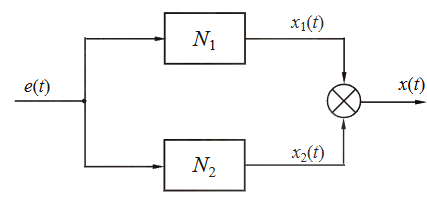
\includegraphics[width = .3\textwidth]{note/nonlinear system/figure/15.png}
\end{center}

此时：
\[
\begin{aligned}
x_1(t) &= N_1(A)A\sin\omega t \\
x_2(t) &= N_2(A)A\sin\omega t \\
x(t) &= x_1(t)+x_2(t) = \bigl(N_1(A)+N_2(A)\bigr)A\sin\omega t
\end{aligned}
\]

\[
N(A)=N_1(A)+N_2(A)
\]

\subsubsection{非线性串联叠加}

非线性的串联可以用以下的示意图表示：
\begin{center}
    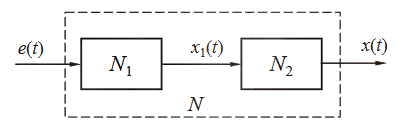
\includegraphics[width = .3\textwidth]{note/nonlinear system/figure/16.png}
\end{center}
由于非线性部分不满足叠加定理，故只能一步一步进行计算，先计算$N_1$模块的输出$x_1(t)$，再计算$N_2$模块的输出，如果还有模块则同理继续进行

\subsection{非线性系统的稳定性}

在讨论非线性系统的稳定性前，我们先由变增益线性系统的稳定性进行引入：

变增益线性系统示意图如下：
\begin{center}
    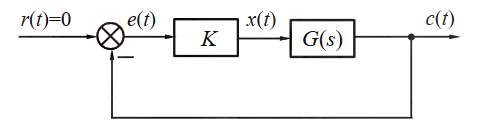
\includegraphics[width = .3\textwidth]{note/nonlinear system/figure/17.png}
\end{center}

设 $G(s)$ 的极点位于左半平面，闭环特征方程：
\[
1+KG(j\omega)=0
\quad \text{或} \quad
G(j\omega)=-\frac{1}{K}
\]

由 Nyquist 稳定判据可知：
\begin{itemize}
    \item 当 $\Gamma_G$ 曲线不包围 $\left(-\frac{1}{K},j0\right)$ 点时，即
    \[
    Z=P-2N=-2N=0
    \]
    时系统闭环稳定；

    \item 当 $\Gamma_G$ 曲线穿过 $\left(-\frac{1}{K},j0\right)$ 点时，系统临界稳定，将产生等幅震荡。

    \item 若设 $K$ 在一定范围内可变，即有 $K_1\le K\le K_2$，
    则 $\left(-\frac{1}{K},j0\right)$ 为复平面实轴上的一段直线，
    若 $\Gamma_G$ 曲线不包围该线段，则系统闭环稳定；
    当 $\Gamma_G$ 曲线包围该线段时，系统闭环不稳定。
\end{itemize}

故我们可以得出以下的非线性系统稳定性判据：

\begin{center}
    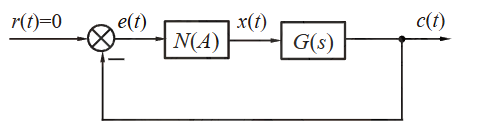
\includegraphics[width = .3\textwidth]{note/nonlinear system/figure/9.png}
\end{center}

假设：描述函数可以作为一个具有复变增益的比例环节；$G(s)$ 具有低通特性，故极点位于左半平面。

闭环特征方程：
\[
1+N(A)G(j\omega)=0
\quad \text{或} \quad
G(j\omega)=-\frac{1}{N(A)}
\]

即
\[
\begin{cases}
|G(j\omega)N(A)|=1 \\
\angle N(A)+\angle G(j\omega)=-180^\circ
\end{cases}
\]

推广的 Nyquist 稳定判据：
\begin{enumerate}
    \item 若线性环节的频率特性 $G(j\omega)$ 的轨迹不包围 $-\dfrac{1}{N(A)}$ 轨迹，如下图(a) 所示，则非线性系统是稳定的，并且 $G(j\omega)$ 离 $-\dfrac{1}{N(A)}$ 越远，系统稳定程度越高。

    \item 若 $G(j\omega)$ 轨迹包围 $-\dfrac{1}{N(A)}$ 轨迹，如下图(b)，则系统是不稳定的，系统将做发散运动。

    \item 若 $G(j\omega)$ 轨迹与 $-\dfrac{1}{N(A)}$ 轨迹有交点，如下图(c)所示，则系统中存在着等幅振荡，其振幅对应交点的振幅和频率。该等幅振荡可能是具有一定稳定性的等幅振荡，即自激振荡；也可能是不稳定的等幅振荡，即在一定条件下等幅振荡发散或收敛。
\end{enumerate}

\begin{center}
    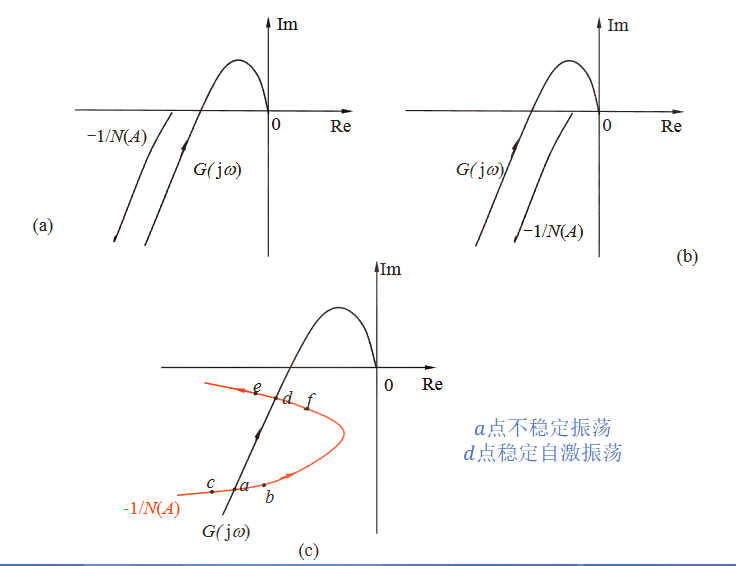
\includegraphics[width = .5\textwidth]{note/nonlinear system/figure/18.png}
\end{center}

从信号的角度分析自振荡产生的条件。在上面图示非线性系统中，若产生自激振荡，
则意味着系统中有一个正弦信号在流通，不妨设非线性环节的输入信号为
\[
e(t)=A\sin\omega t
\]

则非线性环节输出信号基波分量为
\[
x_1(t)=|N(A)|A\sin\!\bigl[\omega t+\angle N(A)\bigr]
\]

而线性部分的输出信号为
\[
c(t)=|G(j\omega)N(A)|A\sin\!\bigl[\omega t+\angle G(j\omega)+\angle N(A)\bigr]
\]

根据系统中存在自振荡的假设，$r(t)=0$，故
\[
e(t)=-c(t)
\]

即
\[
A\sin\omega t
=
-|G(j\omega)N(A)|A\sin\!\bigl[\omega t+\angle G(j\omega)+\angle N(A)\bigr]
\]

不妨以下图为例进行分析：
\begin{center}
    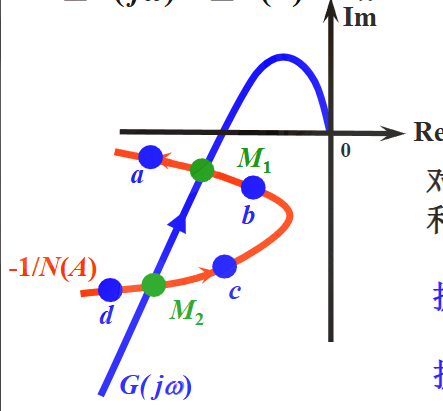
\includegraphics[width = .4\textwidth]{note/nonlinear system/figure/19.png}
\end{center}
其中$M_1$点是稳定的自激振荡点，$M_2$是不稳定的振荡点，对于稳定的自振荡，其振幅和频率是确定的，并可以测量得到。计算时：振幅可由 $-1/N(A)$ 曲线的自变量 $A$ 的大小来确定，振荡频率由 $G(j\omega)$ 曲线的自变量 $\omega$ 来确定。

\begin{example}
    非线性系统结构图如下，已知：
    \begin{center}
        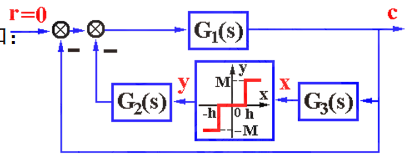
\includegraphics[width = .4\textwidth]{note/nonlinear system/figure/20.png}
    \end{center}
    \[
    \begin{cases}
    G_1(s)=\dfrac{1}{s(s+1)}, \qquad G_2(s)=\dfrac{K}{s} \\[6pt]
    N(A)=\dfrac{4M}{\pi A}\sqrt{1-\left(\dfrac{h}{A}\right)^2},
    \qquad A\ge h
    \end{cases}
    \]
    \begin{enumerate}
        \item $G_3(s) = 1$时，系统是否自振？确定使系统自振的$K$值的范围；求$K = 2$时的自振参数
        \item $G_3(s) = s$时，分析系统的稳定性
    \end{enumerate}
    \tcblower
    先将系统结构图化为典型结构
    \begin{itemize}
        \item 等效变换法：通过方框图法将系统化简：
        \begin{center}
            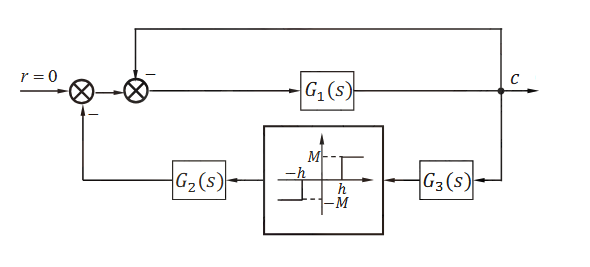
\includegraphics[width = .5\textwidth]{note/nonlinear system/figure/21.png} \\
            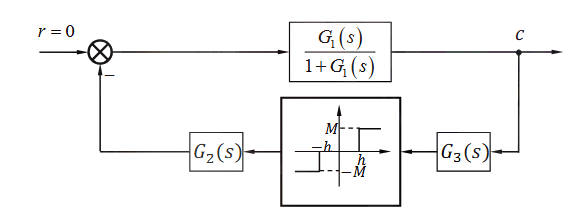
\includegraphics[width = .5\textwidth]{note/nonlinear system/figure/22.png}
        \end{center}
        故$G(s) = \frac{G_1}{1 + G_1} G_2 G_3$
        \item 特征方程法，采用类似线性系统的思想，给出系统的“闭环传递函数为”：
        \begin{align*}
            \Phi(s) = \frac{G_1}{1 + G_1 G_2 G_3 N + G_1}
        \end{align*}
        取出特征方程并化简可得：
        \begin{align*}
            &N\frac{G_1 G_2 G_3}{1 + G_1} = -1 \\
            &G(s) = \frac{G_1}{1 + G_1} G_2 G_3
        \end{align*}
    \end{itemize}
    \begin{enumerate}
        \item $G_3(s)=1$ 时
        \[
        \begin{aligned}
        G(s)
        &= \frac{G_1G_2G_3}{1+G_1} \\
        &= \frac{\dfrac{1}{s(s+1)}\cdot\dfrac{K}{s}\cdot 1}
        {1+\dfrac{1}{s(s+1)}} \\
        &= \frac{K}{s\left(s^2+s+1\right)}
        \end{aligned}
        \]

        \[
        -\frac{1}{N(A)}
        =
        \frac{-\pi A}{4M\sqrt{1-(h/A)^2}}
        =
        \frac{-\pi A^2}{4M\sqrt{A^2-h^2}}
        \]
        当$A \to h$时$\frac{-1}{N(A)} \to -\infty$，当$A\to \infty$时$\frac{-1}{N(A)} \to -\infty$

        由自振条件
        \[
        N(A)\cdot G(j\omega)=-1
        \]

        \[
        \frac{4M}{\pi A}\sqrt{1-\left(\frac{h}{A}\right)^2}
        \cdot
        \frac{K}{j\omega(1-\omega^2+j\omega)}
        =-1
        \]

        \[
        \begin{aligned}
        \frac{4MK}{\pi A}\sqrt{1-\left(\frac{h}{A}\right)^2}
        &= -j\omega(1-\omega^2+j\omega) \\
        &= \omega^2-j\omega(1-\omega^2)
        \end{aligned}
        \]
        观察实部和虚部可得：
        \[
        \begin{cases}
        \omega=1, \\[4pt]
        \dfrac{4K}{\pi A^2}\sqrt{A^2-1}=1\rightarrow\sqrt{A^2-1}=\dfrac{\pi A^2}{4K}.
        \end{cases}
        \]
        由第二条式子可以解得$A^2 = \frac{1 \pm \sqrt{1 - 4 (\pi / 4K)^2}}{2(\pi/4K)^2}$，所以有解的条件为：$K \ge \frac{\pi}{2}$，当$K= 2$时可以算出$A^2 = 5.25$或$1.1122$，故
        \[
        \begin{cases}
        A_1=2.29, \\
        A_2=1.055.
        \end{cases}
        \]
        由自激振荡的条件可以知道需要取大者，所以可以解得：
        \[
        \begin{cases}
        A=2.29, \\
        \omega=1.
        \end{cases}
        \]
        \item $G_3(s)=s$ 时
        \[
        \begin{aligned}
        G(s)
        &= \frac{G_1G_2G_3}{1+G_1} \\
        &= \frac{\dfrac{1}{s(s+1)}\cdot\dfrac{K}{s}\cdot s}
        {1+\dfrac{1}{s(s+1)}} \\
        &= \frac{K}{s^2+s+1}
        \end{aligned}
        \]
        画出图像如下，可以看出此时系统稳定
        \begin{center}
            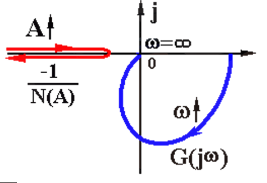
\includegraphics[width = .4\textwidth]{note/nonlinear system/figure/23.png}
        \end{center}
    \end{enumerate}
\end{example}

\section{相平面法}
\subsection{相平面法的基本概念}
相平面法是分析非线性系统稳定性的一个重要工具。对于一个二阶非线性系统，我们可以将其状态变量$x$和$\dot{x}$分别作为横轴和纵轴，在平面上描绘出系统的轨迹，这个平面就被称为相平面。在相平面上绘制出来的轨迹叫做相轨迹

我们可以给出相平面的一些性质如下：
\begin{property}[相平面的一些性质]
    \begin{enumerate}
        \item 相轨迹的斜率：$\frac{\mathrm{d}\dot{x}}{\mathrm{d}x}=\frac{-f(x,\dot{x})}{\dot{x}}$
        \item 相轨迹的就奇点（平衡点）：满足$\ddot{x} = \dot{x} = 0$的点，即相轨迹上的斜率不确定点，在$x$轴上，对于线性定常系统，原点是唯一的平衡点
        \item 相轨迹的运动方向：由斜率的符号可以确定相轨迹的运动方向
        \item 相轨迹通过横轴的方向：相轨迹以90°的角度穿过横轴
        \item 相轨迹的对称性：如果系统的函数$f(x,\dot{x})$是$x$的奇函数，那么相轨迹关于$\dot{x}$轴对称；如果$f(x,\dot{x})$是$\dot{x}$的偶函数，那么相轨迹关于$x$轴对称。
    \end{enumerate}
\end{property}

\subsection{相轨迹的绘制}

\subsubsection{解析法}
解析法是通过求解系统的微分方程来得到相轨迹的表达式，从而绘制出相轨迹，我们有以下两种方法：
\begin{enumerate}
    \item 直接积分法：通过将系统的微分方程进行积分，得到相轨迹的表达式，从而绘制出相轨迹。
    \item 消去时间变量$t$：通过将系统的微分方程中的时间变量$t$消去，得到一个关于$x$和$\dot{x}$的方程，从而绘制出相轨迹。
\end{enumerate}

\subsubsection{等倾线法}
对于二阶系统
\[
\ddot{x}+f(x,\dot{x})=0,
\]
其斜率方程为：
\[
\frac{d\dot{x}}{dx}=-\frac{f(x,\dot{x})}{\dot{x}}
\]

该方程给出了相轨迹在相平面上任一点 $(x,\dot{x})$ 处切线的斜率。取相轨迹切线的斜率为某一常数 $\alpha$，得：
\[
\alpha=\frac{d\dot{x}}{dx}=-\frac{f(x,\dot{x})}{\dot{x}}
\]

也就是说，相平面上满足该方程的点 $(x,\dot{x})$，其所对应的相轨迹在该点处切线的斜率为 $\alpha$。如果 $\dot{x}\neq 0$，则：
\[
\alpha\dot{x}+f(x,\dot{x})=0
\]

该方程称为二阶系统的等倾线方程。

\begin{itemize}
    \item 二阶系统的等倾线方程可将系统方程 $\ddot{x}+f(x,\dot{x})=0$ 中 $\ddot{x}$ 替换为 $\alpha\dot{x}$ 得到。
    \item 根据等倾线方程，可在相平面的各条相轨迹上求出具有同一斜率的点 $(x,\dot{x})$，将这些点连接起来，由此得到的等斜率轨迹亦称为等倾线。
\end{itemize}

对于二阶线性系统，
\[
\ddot{x}+a\dot{x}+bx=0
\]

其等倾线为直线，其方程为：
\[
\dot{x}=-\frac{b}{a+\alpha}x
\]

其中 $\alpha$ 为相轨迹切线的斜率，而该等倾线的斜率为：
\[
k=-\frac{b}{a+\alpha}
\]

考虑一类等倾线：等倾线的斜率与相轨迹切线斜率相等。这类等倾线也是相轨迹。
\[
k=-\frac{b}{a+k}
\]

\[
k^2+ak+b=0
\]

\begin{itemize}
    \item 特殊等倾线的斜率是系统的极点。
    \item 具有复数极点的二阶线性系统不存在这样的特殊等倾线。
\end{itemize}

当 $b<0$ 时，系统的两个极点为：
\[
s_1=-\frac{a+\sqrt{a^2-4b}}{2}<0,
\qquad
s_2=-\frac{a-\sqrt{a^2-4b}}{2}>0
\]

\subsubsection{线性二阶系统的相轨迹}

我们研究以下这种系统的不同情况：
\begin{align*}
    \ddot{x} + 2 \xi \omega_n \dot{x} + \omega_n^2 x = 0
\end{align*}

\begin{enumerate}
    \item $0<\xi<1$时，系统有两个实部为负的共轭复根，系统的奇点为稳定焦点，如下图所示：
    \begin{center}
        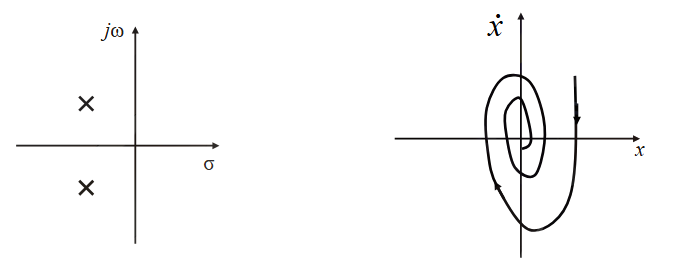
\includegraphics[width = .5\textwidth]{note/nonlinear system/figure/24.png}
    \end{center}
    \item $-1<\xi<0$时，系统有两个实部为正的共轭复根，系统的奇点为不稳定焦点，如下图所示：
    \begin{center}
        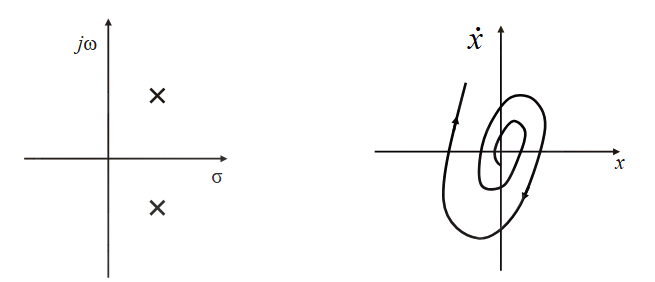
\includegraphics[width = .5\textwidth]{note/nonlinear system/figure/25.png}
    \end{center}
    \item $\xi>1$时，系统有两个负实根，相轨迹中有两条特殊等倾线，系统的奇点为稳定节点，如下图所示：
    \begin{center}
        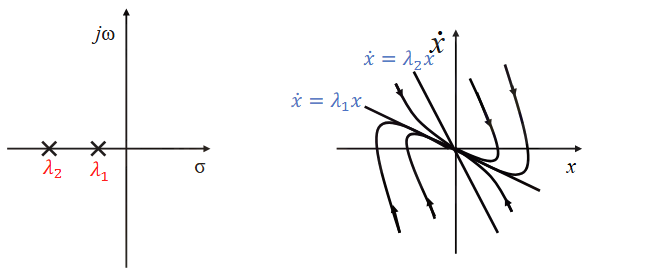
\includegraphics[width = .5\textwidth]{note/nonlinear system/figure/26.png}
    \end{center}
    \item $\xi<-1$时，系统有两个正实根，相轨迹中有两条特殊等倾线，系统的奇点为不稳定节点，如下图所示：
    \begin{center}
        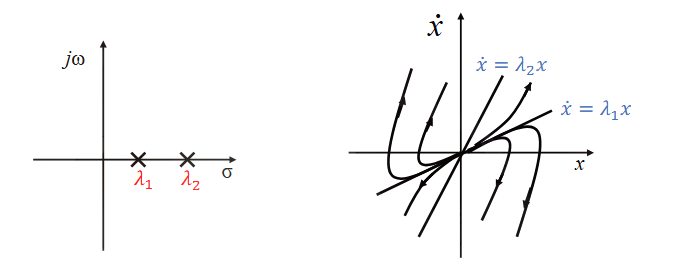
\includegraphics[width = .5\textwidth]{note/nonlinear system/figure/27.png}
    \end{center}
    \item $\xi = 0$时，系统有两个实部为零的共轭复根，系统的奇点为中心点，相轨迹为以奇点为中心的同心椭圆，如下图所示：
    \begin{center}
        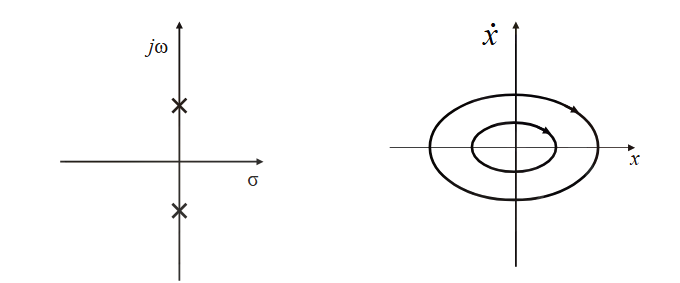
\includegraphics[width = .5\textwidth]{note/nonlinear system/figure/28.png}
    \end{center}
    \item 考虑另一个二阶线性系统：$\ddot{x} + 2\xi \omega_n \dot{x} - \omega_n^2 x = 0$，此系统含有两个异号实根，相轨迹有两条特殊等倾线，系统的奇点为鞍点，如下图所示：
    \begin{center}
        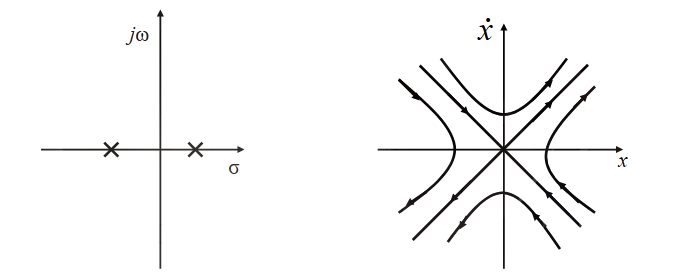
\includegraphics[width = .5\textwidth]{note/nonlinear system/figure/29.png}
    \end{center}
\end{enumerate}

以上的六种情况可以总结为以下这一张图：
\begin{center}
    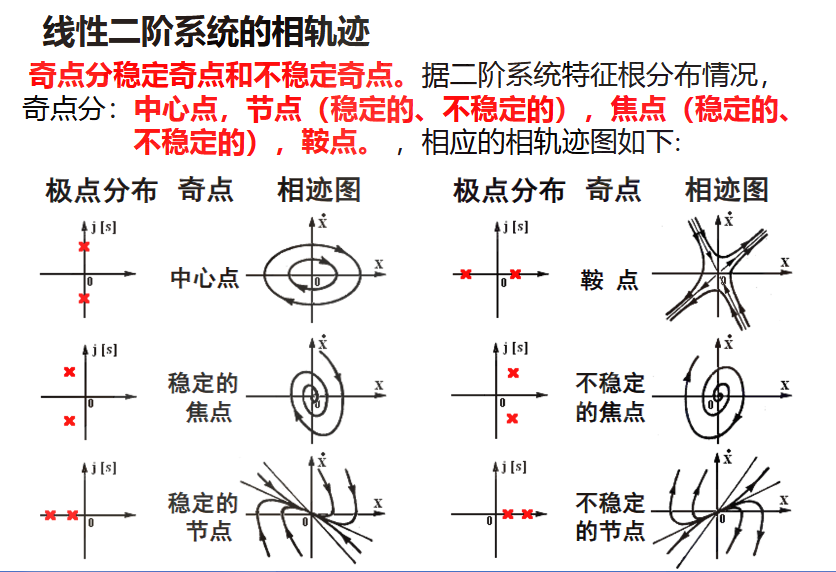
\includegraphics[width = .6\textwidth]{note/nonlinear system/figure/30.png}
\end{center}

\subsubsection{非线性系统的相轨迹}

对于非线性系统，平衡状态和平衡状态附近系统的运动形式以及极限环的存在
制约着整个系统的运动特性。对于非线性系统的各个平衡点，若描述非线性过程的
非线性函数解析时，可以通过平衡点处的线性化方程，基于线性系统特征根的分布，
确定奇点的类型，进而确定平衡点附近相轨迹的运动形式。

\begin{enumerate}
    \item 若$f(x,\dot{x})$解析，则我们可以将方程$\ddot{x} + f(x,\dot{x}) = 0$在奇点$(x_0,\dot{x}_0)$处展开：
    \[
    \Delta \ddot{x}
    = - \left. \frac{\partial f(x,\dot{x})}{\partial x} \right|_{\substack{x=x_0\\ \dot{x}=\dot{x}_0}} \Delta x
    - \left. \frac{\partial f(x,\dot{x})}{\partial \dot{x}} \right|_{\substack{x=x_0\\ \dot{x}=\dot{x}_0}} \Delta \dot{x}
    \]
    此时微分方程就可以近似写为一个二阶线性方程：
    \[
         \ddot{x}
     + \left. \frac{\partial f(x,\dot{x})}{\partial x} \right|_{\substack{x=x_0\\ \dot{x}=\dot{x}_0}}  x
    + \left. \frac{\partial f(x,\dot{x})}{\partial \dot{x}} \right|_{\substack{x=x_0\\ \dot{x}=\dot{x}_0}}  \dot{x} = 0
    \]
    \item 如果$f(x,\dot{x})$不解析，可以根据非线性特性将相平面划分成若干区域
    \begin{itemize}
        \item 在各区域内，非线性方程$f(x,\dot{x})$可满足解析条件或可以表示为线性微分方程
        \item 若某区域内非线性方程可线性化，奇点类型即决定该区域系统运动的形态
        \item 若对应奇点位于本区域内，称为实奇点，若对应奇点位于其他区域，称为虚奇点
    \end{itemize}
    \item 当非线性系统存在多个奇点时，奇点类型只决定奇点附近相轨迹的运动形式。
    \item 整个系统的相轨迹，特别是离奇点较远的部分，还取决于多个奇点的共同作用。
    \item 有时会产生特殊的相轨迹，将相平面划分为具有不同运动特点的多个区域。这种特殊的相轨迹称为奇线。
    \item 最常见的奇线是极限环。极限环把相平面的某个区域划分为内部平面和外部平面部分。
    \begin{itemize}
        \item 极限环是非线性系统的特有现象，表示系统稳态运动的、孤立的封闭曲线。
        \item 把相平面划分为具有不同运动特点的各个区域。
        \item 收敛于该极限环，则极限环称为稳定极限环。系统呈现稳定的自振。
        \item 一些复杂的非线性控制系统可能出现两个或两个以上极限环。
        \item 该非线性系统的工作状态，不仅取决于初始条件，也取决于扰动大小。
        \item 只有稳定的极限环才能在实验中被观察到。不稳定或半稳定的极限环无法在实验中观察到
    \end{itemize}
    \item 常见非线性特性多数可用分段直线来表示，或者本身就是分段线性的。
    \item 对于含有这些非线性特性的一大类非线性系统，由于不满足解析条件，无法采用小扰动线性化方法。
    \item 根据非线性的分段特点，将相平面分成若干区域进行研究，可使非线性微分方程在各个区域表现为线性微分方程，再应用线性系统的相平面分析方法，则问题将迎刃而解。
    \item 这一类非线性特性曲线的折线的各转折点，构成了相平面区域的分界线，称为\textcolor{red}{开关线}。
\end{enumerate}

\begin{example}
    系统如下，已知
\[
\begin{cases}
c(0)=0,\\
r(t)=4\times 1(t),
\end{cases}
\]
确定开关线方程、奇点位置和类型，绘制相轨迹 $(e,\dot{e})$ 图。
\begin{center}
    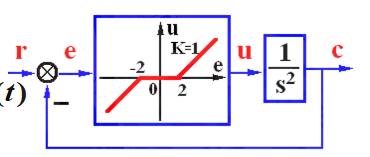
\includegraphics[width = .5\textwidth]{note/nonlinear system/figure/31.png}
\end{center}
\tcblower
线性部分：
\[
\frac{C(s)}{U(s)}=\frac{1}{s^2}
\quad \Rightarrow \quad
\ddot{c}(t)=u(t)
\]

非线性部分：
\[
u=
\begin{cases}
0, & |e|\leq 2 \quad (\mathrm{I})\\
e-2, & e>2 \quad (\mathrm{II})\\
e+2, & e<-2 \quad (\mathrm{III})
\end{cases}
\]

开关线方程：
\[
\begin{cases}
e=2,\\
e=-2.
\end{cases}
\]

综合点：
\[
e=r-c=4-c
\]
\[
\begin{cases}
c=4-e,\\
\dot{c}=-\dot{e},\\
\ddot{c}=-\ddot{e}.
\end{cases}
\]

因此
\[
\ddot{e}
=-\ddot{c}
=-u
=
\begin{cases}
0, & |e|\leq 2 \quad (\mathrm{I})\\
2-e, & e>2 \quad (\mathrm{II})\\
-2-e, & e<-2 \quad (\mathrm{III})
\end{cases}
\]
因此可以画出以下这个表：
\[
\begin{array}{c|c|c|c|c|c}
\text{区域} & \text{运动方程} & \text{奇点} & \text{特征方程} & \text{极点} & \text{奇点性质} \\
\hline
\mathrm{I} & \ddot{e}=0 & \dot{e}=0 & s^2=0 & s=0 & \\
\mathrm{II} & \ddot{e}+e-2=0 & (2,0) & s^2+1=0 & s=\pm j & \text{中心点} \\
\mathrm{III} & \ddot{e}+e+2=0 & (-2,0) & s^2+1=0 & s=\pm j & \text{中心点}
\end{array}
\]
所以相轨迹为：
\[
\begin{cases}
(\mathrm{I}) \quad \ddot{e}=0,\quad \dot{e}=C, \quad \text{水平线},\\
(\mathrm{II}) \quad \text{以 } (2,0) \text{ 为中心的圆},\\
(\mathrm{III}) \quad \text{以 } (-2,0) \text{ 为中心的圆}.
\end{cases}
\]
画出相轨迹如下：
\begin{center}
    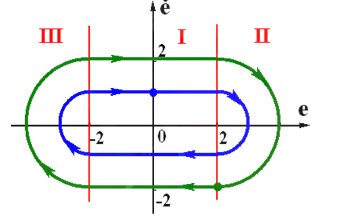
\includegraphics[width = .4\textwidth]{note/nonlinear system/figure/32.png}
\end{center}
\end{example}

\begin{example}
    系统如下，在 $(c,\dot{c})$ 平面上分析系统的自由响应运动。
    \begin{center}
        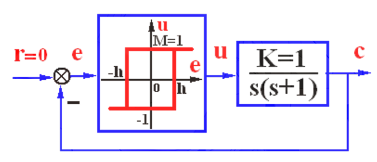
\includegraphics[width = .4\textwidth]{note/nonlinear system/figure/33.png}
    \end{center}
    \tcblower
线性部分：
\[
\frac{C(s)}{U(s)}=\frac{1}{s^2+s}
\]

\[
\ddot{c}+\dot{c}=u
\]

非线性部分：
\[
u=
\begin{cases}
1,
&
\begin{cases}
e>h,\\
e>-h,\ \dot{e}<0,
\end{cases}
\\[6pt]
-1,
&
\begin{cases}
e<-h,\\
e<h,\ \dot{e}>0.
\end{cases}
\end{cases}
\]

比较点：
\[
e=r-c
\]

自由响应时 $r=0$，故
\[
e=-c,\qquad \dot{e}=-\dot{c}
\]

整理：
\[
\ddot{c}+\dot{c}=u=
\begin{cases}
1,
&
\begin{cases}
c<-h,\\
c<h,\ \dot{c}>0,
\end{cases}
\\[6pt]
-1,
&
\begin{cases}
c>h,\\
c>-h,\ \dot{c}<0.
\end{cases}
\end{cases}
\]
所以可以画出开关线如下：
\begin{center}
    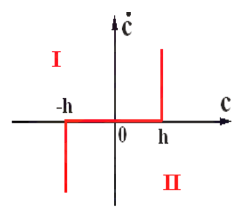
\includegraphics[width = .4\textwidth]{note/nonlinear system/figure/34.png}
\end{center}
\[
(\mathrm{I})\quad
\ddot{c}
=
\dot{c}\frac{d\dot{c}}{dc}
=
\alpha \dot{c}
=
1-\dot{c}
\qquad
\text{等倾斜线 }
\dot{c}=\frac{1}{1+\alpha}
\]

\[
(\mathrm{II})\quad
\ddot{c}
=
\dot{c}\frac{d\dot{c}}{dc}
=
\alpha \dot{c}
=
-1-\dot{c}
\qquad
\text{等倾斜线 }
\dot{c}=\frac{-1}{1+\alpha}
\]
根据上面的式子可以给出以下这个表：
\[
\begin{array}{cc|cccccccc}
\multicolumn{2}{c|}{\alpha}
& -\frac{1}{2} & -\frac{1}{3} & 0 & 1 & \infty & -3 & -2 & -\frac{3}{2} \\
\hline
\mathrm{I} & \frac{1}{1+\alpha}
& 2 & \frac{3}{2} & 1 & \frac{1}{2} & 0 & -\frac{1}{2} & -1 & -2 \\
\mathrm{II} & -\frac{1}{1+\alpha}
& -2 & -\frac{3}{2} & -1 & -\frac{1}{2} & 0 & \frac{1}{2} & 1 & 2
\end{array}
\]
所以可以画出系统的相轨迹如下：
\begin{center}
    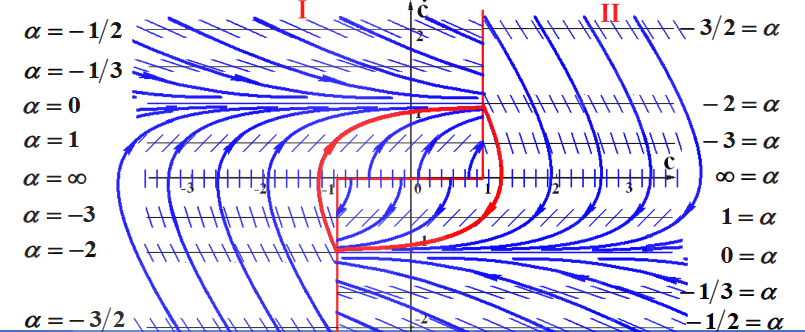
\includegraphics[width = .6\textwidth]{note/nonlinear system/figure/35.png}
\end{center}
\end{example}
